\documentclass{standalone}
\usepackage{tikz}
\usetikzlibrary{patterns, positioning}

\begin{document}
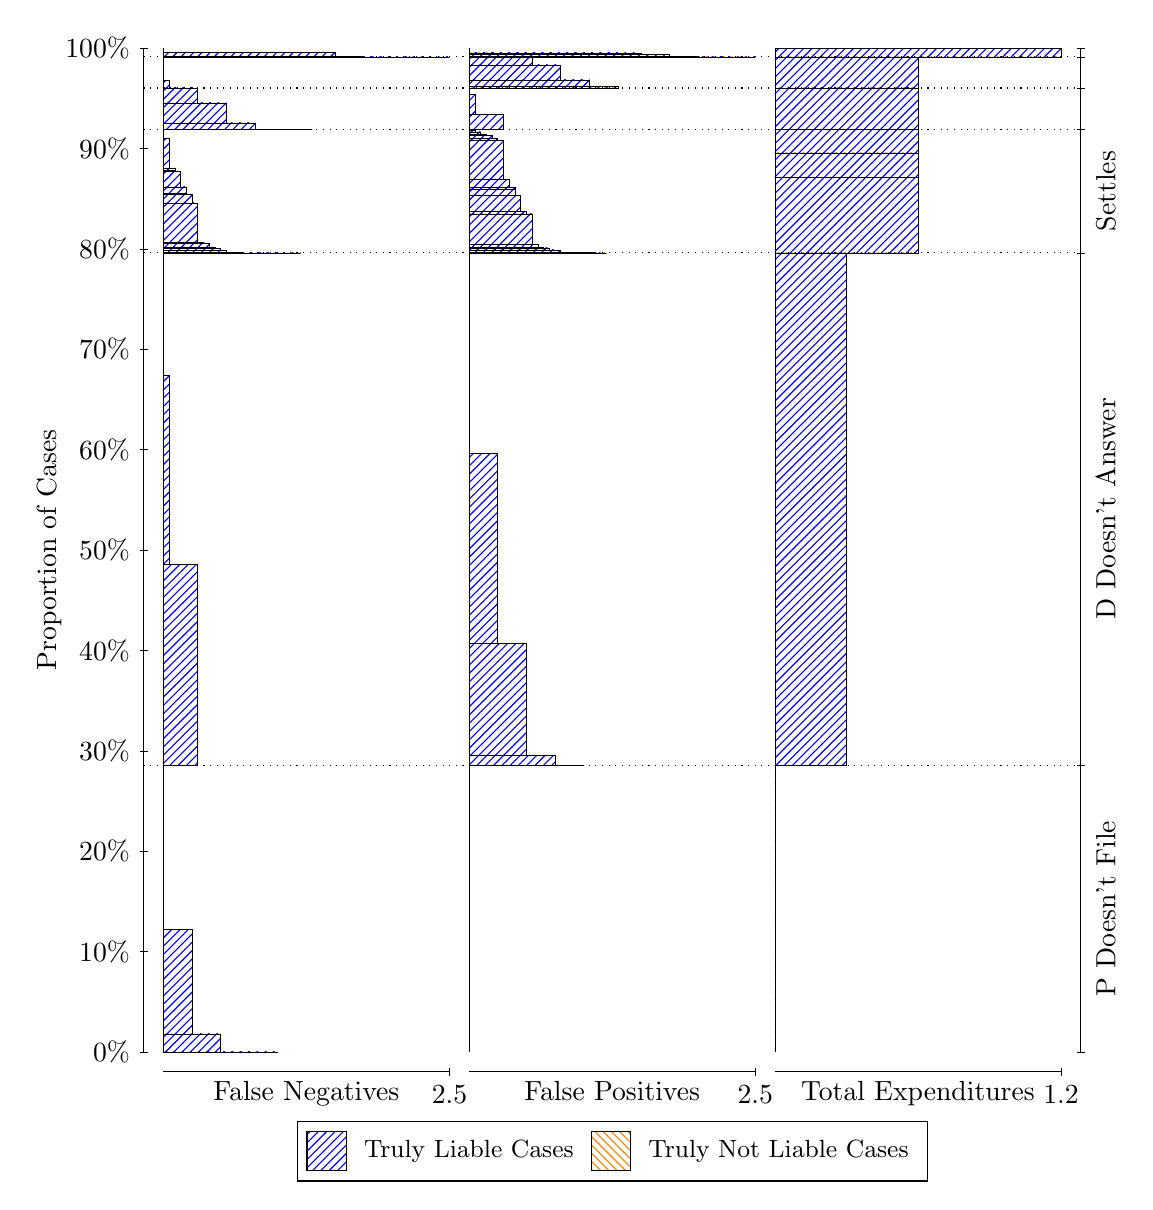
\begin{tikzpicture}
\draw[black, very thin] (1.5,1.75) -- (1.5,14.5);
\node[rotate=90, anchor=center] at (0.3, 8.125) {Proportion of Cases};
\draw[black, very thin] (1.45,1.75) -- (1.55,1.75);
\node[anchor=east] at (1.45, 1.75) {0\%};
\draw[black, very thin] (1.45,3.025) -- (1.55,3.025);
\node[anchor=east] at (1.45, 3.025) {10\%};
\draw[black, very thin] (1.45,4.3) -- (1.55,4.3);
\node[anchor=east] at (1.45, 4.3) {20\%};
\draw[black, very thin] (1.45,5.575) -- (1.55,5.575);
\node[anchor=east] at (1.45, 5.575) {30\%};
\draw[black, very thin] (1.45,6.85) -- (1.55,6.85);
\node[anchor=east] at (1.45, 6.85) {40\%};
\draw[black, very thin] (1.45,8.125) -- (1.55,8.125);
\node[anchor=east] at (1.45, 8.125) {50\%};
\draw[black, very thin] (1.45,9.4) -- (1.55,9.4);
\node[anchor=east] at (1.45, 9.4) {60\%};
\draw[black, very thin] (1.45,10.675) -- (1.55,10.675);
\node[anchor=east] at (1.45, 10.675) {70\%};
\draw[black, very thin] (1.45,11.95) -- (1.55,11.95);
\node[anchor=east] at (1.45, 11.95) {80\%};
\draw[black, very thin] (1.45,13.225) -- (1.55,13.225);
\node[anchor=east] at (1.45, 13.225) {90\%};
\draw[black, very thin] (1.45,14.5) -- (1.55,14.5);
\node[anchor=east] at (1.45, 14.5) {100\%};

\draw[black, very thin] (13.4,1.75) -- (13.4,14.5);
\draw[black, very thin] (13.35,1.75) -- (13.45,1.75);
\node[anchor=west] at (13.35, 1.75) {};
\draw[black, very thin] (13.35,5.3919) -- (13.45,5.3919);
\node[anchor=west] at (13.35, 5.3919) {};
\draw[black, very thin] (13.35,11.899) -- (13.45,11.899);
\node[anchor=west] at (13.35, 11.899) {};
\draw[black, very thin] (13.35,13.467) -- (13.45,13.467);
\node[anchor=west] at (13.35, 13.467) {};
\draw[black, very thin] (13.35,13.993) -- (13.45,13.993);
\node[anchor=west] at (13.35, 13.993) {};
\draw[black, very thin] (13.35,14.387) -- (13.45,14.387);
\node[anchor=west] at (13.35, 14.387) {};
\draw[black, very thin] (13.35,14.5) -- (13.45,14.5);
\node[anchor=west] at (13.35, 14.5) {};

\draw[black, very thin, pattern color=blue, pattern=north east lines] (1.75,1.75) rectangle (3.2033,1.75);
\draw[black, very thin, pattern color=blue, pattern=north east lines] (1.75,1.75) rectangle (2.84,1.7519);
\draw[black, very thin, pattern color=blue, pattern=north east lines] (1.75,1.7519) rectangle (2.4767,1.9795);
\draw[black, very thin, pattern color=blue, pattern=north east lines] (1.75,1.9795) rectangle (2.1133,3.3082);
\draw[black, very thin, pattern color=orange, pattern=north west lines] (1.75,3.3082) rectangle (1.75,3.3082);
\draw[black, very thin, pattern color=blue, pattern=north east lines] (1.75,3.3082) rectangle (1.75,5.3919);
\draw[black, very thin, pattern color=blue, pattern=north east lines] (1.75,5.3919) rectangle (2.186,7.9404);
\draw[black, very thin, pattern color=blue, pattern=north east lines] (1.75,7.9404) rectangle (1.8227,10.35);
\draw[black, very thin, pattern color=orange, pattern=north west lines] (1.75,10.35) rectangle (1.75,10.35);
\draw[black, very thin, pattern color=blue, pattern=north east lines] (1.75,10.35) rectangle (1.75,11.899);
\draw[black, very thin, pattern color=blue, pattern=north east lines] (1.75,11.899) rectangle (3.494,11.899);
\draw[black, very thin, pattern color=blue, pattern=north east lines] (1.75,11.899) rectangle (3.3487,11.899);
\draw[black, very thin, pattern color=blue, pattern=north east lines] (1.75,11.899) rectangle (3.2033,11.899);
\draw[black, very thin, pattern color=blue, pattern=north east lines] (1.75,11.899) rectangle (3.1307,11.899);
\draw[black, very thin, pattern color=blue, pattern=north east lines] (1.75,11.899) rectangle (3.058,11.899);
\draw[black, very thin, pattern color=blue, pattern=north east lines] (1.75,11.899) rectangle (3.058,11.899);
\draw[black, very thin, pattern color=blue, pattern=north east lines] (1.75,11.899) rectangle (2.9853,11.899);
\draw[black, very thin, pattern color=blue, pattern=north east lines] (1.75,11.899) rectangle (2.9127,11.899);
\draw[black, very thin, pattern color=blue, pattern=north east lines] (1.75,11.899) rectangle (2.84,11.899);
\draw[black, very thin, pattern color=blue, pattern=north east lines] (1.75,11.899) rectangle (2.7673,11.9);
\draw[black, very thin, pattern color=blue, pattern=north east lines] (1.75,11.9) rectangle (2.6947,11.9);
\draw[black, very thin, pattern color=blue, pattern=north east lines] (1.75,11.9) rectangle (2.6947,11.901);
\draw[black, very thin, pattern color=blue, pattern=north east lines] (1.75,11.901) rectangle (2.622,11.901);
\draw[black, very thin, pattern color=blue, pattern=north east lines] (1.75,11.901) rectangle (2.622,11.905);
\draw[black, very thin, pattern color=blue, pattern=north east lines] (1.75,11.905) rectangle (2.5493,11.93);
\draw[black, very thin, pattern color=blue, pattern=north east lines] (1.75,11.93) rectangle (2.4767,11.961);
\draw[black, very thin, pattern color=blue, pattern=north east lines] (1.75,11.961) rectangle (2.404,11.962);
\draw[black, very thin, pattern color=blue, pattern=north east lines] (1.75,11.962) rectangle (2.404,11.971);
\draw[black, very thin, pattern color=blue, pattern=north east lines] (1.75,11.971) rectangle (2.3313,11.972);
\draw[black, very thin, pattern color=blue, pattern=north east lines] (1.75,11.972) rectangle (2.3313,12.018);
\draw[black, very thin, pattern color=blue, pattern=north east lines] (1.75,12.018) rectangle (2.3313,12.018);
\draw[black, very thin, pattern color=blue, pattern=north east lines] (1.75,12.018) rectangle (2.2587,12.02);
\draw[black, very thin, pattern color=blue, pattern=north east lines] (1.75,12.02) rectangle (2.2587,12.033);
\draw[black, very thin, pattern color=blue, pattern=north east lines] (1.75,12.033) rectangle (2.186,12.533);
\draw[black, very thin, pattern color=blue, pattern=north east lines] (1.75,12.533) rectangle (2.1133,12.64);
\draw[black, very thin, pattern color=blue, pattern=north east lines] (1.75,12.64) rectangle (2.0407,12.654);
\draw[black, very thin, pattern color=blue, pattern=north east lines] (1.75,12.654) rectangle (2.0407,12.736);
\draw[black, very thin, pattern color=blue, pattern=north east lines] (1.75,12.736) rectangle (1.968,12.736);
\draw[black, very thin, pattern color=blue, pattern=north east lines] (1.75,12.736) rectangle (1.968,12.935);
\draw[black, very thin, pattern color=blue, pattern=north east lines] (1.75,12.935) rectangle (1.968,12.938);
\draw[black, very thin, pattern color=blue, pattern=north east lines] (1.75,12.938) rectangle (1.8953,12.952);
\draw[black, very thin, pattern color=blue, pattern=north east lines] (1.75,12.952) rectangle (1.8953,12.971);
\draw[black, very thin, pattern color=blue, pattern=north east lines] (1.75,12.971) rectangle (1.8227,13.356);
\draw[black, very thin, pattern color=orange, pattern=north west lines] (1.75,13.356) rectangle (1.75,13.356);
\draw[black, very thin, pattern color=blue, pattern=north east lines] (1.75,13.356) rectangle (1.75,13.467);
\draw[black, very thin, pattern color=blue, pattern=north east lines] (1.75,13.467) rectangle (3.6393,13.467);
\draw[black, very thin, pattern color=blue, pattern=north east lines] (1.75,13.467) rectangle (3.276,13.469);
\draw[black, very thin, pattern color=blue, pattern=north east lines] (1.75,13.469) rectangle (2.9127,13.548);
\draw[black, very thin, pattern color=blue, pattern=north east lines] (1.75,13.548) rectangle (2.5493,13.804);
\draw[black, very thin, pattern color=blue, pattern=north east lines] (1.75,13.804) rectangle (2.186,13.993);
\draw[black, very thin, pattern color=orange, pattern=north west lines] (1.75,13.993) rectangle (1.75,13.993);
\draw[black, very thin, pattern color=blue, pattern=north east lines] (1.75,13.993) rectangle (2.186,13.994);
\draw[black, very thin, pattern color=blue, pattern=north east lines] (1.75,13.994) rectangle (1.8227,14.093);
\draw[black, very thin, pattern color=orange, pattern=north west lines] (1.75,14.093) rectangle (1.75,14.093);
\draw[black, very thin, pattern color=blue, pattern=north east lines] (1.75,14.093) rectangle (1.75,14.387);
\draw[black, very thin, pattern color=blue, pattern=north east lines] (1.75,14.387) rectangle (5.3833,14.387);
\draw[black, very thin, pattern color=blue, pattern=north east lines] (1.75,14.387) rectangle (5.02,14.387);
\draw[black, very thin, pattern color=blue, pattern=north east lines] (1.75,14.387) rectangle (4.6567,14.388);
\draw[black, very thin, pattern color=blue, pattern=north east lines] (1.75,14.388) rectangle (4.2933,14.398);
\draw[black, very thin, pattern color=blue, pattern=north east lines] (1.75,14.398) rectangle (3.93,14.446);
\draw[black, very thin, pattern color=blue, pattern=north east lines] (1.75,14.446) rectangle (3.5667,14.448);
\draw[black, very thin, pattern color=blue, pattern=north east lines] (1.75,14.448) rectangle (3.2033,14.448);
\draw[black, very thin, pattern color=blue, pattern=north east lines] (1.75,14.448) rectangle (2.404,14.448);
\draw[black, very thin, pattern color=blue, pattern=north east lines] (1.75,14.448) rectangle (2.0407,14.448);
\draw[black, very thin, pattern color=orange, pattern=north west lines] (1.75,14.448) rectangle (1.75,14.448);
\draw[black, very thin, pattern color=blue, pattern=north east lines] (1.75,14.448) rectangle (1.75,14.5);
\draw[black, very thin, pattern color=orange, pattern=north west lines] (5.6333,1.75) rectangle (5.6333,1.75);
\draw[black, very thin, pattern color=blue, pattern=north east lines] (5.6333,1.75) rectangle (5.6333,5.3919);
\draw[black, very thin, pattern color=orange, pattern=north west lines] (5.6333,5.3919) rectangle (7.0867,5.3919);
\draw[black, very thin, pattern color=blue, pattern=north east lines] (5.6333,5.3919) rectangle (7.0867,5.3924);
\draw[black, very thin, pattern color=blue, pattern=north east lines] (5.6333,5.3924) rectangle (6.7233,5.5215);
\draw[black, very thin, pattern color=blue, pattern=north east lines] (5.6333,5.5215) rectangle (6.36,6.9408);
\draw[black, very thin, pattern color=blue, pattern=north east lines] (5.6333,6.9408) rectangle (5.9967,9.35);
\draw[black, very thin, pattern color=blue, pattern=north east lines] (5.6333,9.35) rectangle (5.6333,11.899);
\draw[black, very thin, pattern color=orange, pattern=north west lines] (5.6333,11.899) rectangle (7.3773,11.899);
\draw[black, very thin, pattern color=blue, pattern=north east lines] (5.6333,11.899) rectangle (7.3773,11.899);
\draw[black, very thin, pattern color=orange, pattern=north west lines] (5.6333,11.899) rectangle (7.232,11.899);
\draw[black, very thin, pattern color=blue, pattern=north east lines] (5.6333,11.899) rectangle (7.232,11.9);
\draw[black, very thin, pattern color=orange, pattern=north west lines] (5.6333,11.9) rectangle (7.0867,11.9);
\draw[black, very thin, pattern color=blue, pattern=north east lines] (5.6333,11.9) rectangle (7.0867,11.902);
\draw[black, very thin, pattern color=blue, pattern=north east lines] (5.6333,11.902) rectangle (7.014,11.903);
\draw[black, very thin, pattern color=orange, pattern=north west lines] (5.6333,11.903) rectangle (6.9413,11.903);
\draw[black, very thin, pattern color=blue, pattern=north east lines] (5.6333,11.903) rectangle (6.9413,11.907);
\draw[black, very thin, pattern color=blue, pattern=north east lines] (5.6333,11.907) rectangle (6.8687,11.907);
\draw[black, very thin, pattern color=orange, pattern=north west lines] (5.6333,11.907) rectangle (6.796,11.907);
\draw[black, very thin, pattern color=blue, pattern=north east lines] (5.6333,11.907) rectangle (6.796,11.931);
\draw[black, very thin, pattern color=blue, pattern=north east lines] (5.6333,11.931) rectangle (6.7233,11.936);
\draw[black, very thin, pattern color=orange, pattern=north west lines] (5.6333,11.936) rectangle (6.6507,11.936);
\draw[black, very thin, pattern color=blue, pattern=north east lines] (5.6333,11.936) rectangle (6.6507,11.961);
\draw[black, very thin, pattern color=blue, pattern=north east lines] (5.6333,11.961) rectangle (6.578,11.969);
\draw[black, very thin, pattern color=blue, pattern=north east lines] (5.6333,11.969) rectangle (6.5053,11.97);
\draw[black, very thin, pattern color=orange, pattern=north west lines] (5.6333,11.97) rectangle (6.5053,11.97);
\draw[black, very thin, pattern color=blue, pattern=north east lines] (5.6333,11.97) rectangle (6.5053,12.01);
\draw[black, very thin, pattern color=blue, pattern=north east lines] (5.6333,12.01) rectangle (6.4327,12.395);
\draw[black, very thin, pattern color=orange, pattern=north west lines] (5.6333,12.395) rectangle (6.36,12.395);
\draw[black, very thin, pattern color=blue, pattern=north east lines] (5.6333,12.395) rectangle (6.36,12.428);
\draw[black, very thin, pattern color=blue, pattern=north east lines] (5.6333,12.428) rectangle (6.2873,12.63);
\draw[black, very thin, pattern color=orange, pattern=north west lines] (5.6333,12.63) rectangle (6.2147,12.63);
\draw[black, very thin, pattern color=blue, pattern=north east lines] (5.6333,12.63) rectangle (6.2147,12.712);
\draw[black, very thin, pattern color=blue, pattern=north east lines] (5.6333,12.712) rectangle (6.2147,12.726);
\draw[black, very thin, pattern color=blue, pattern=north east lines] (5.6333,12.726) rectangle (6.142,12.727);
\draw[black, very thin, pattern color=blue, pattern=north east lines] (5.6333,12.727) rectangle (6.142,12.833);
\draw[black, very thin, pattern color=blue, pattern=north east lines] (5.6333,12.833) rectangle (6.0693,13.333);
\draw[black, very thin, pattern color=blue, pattern=north east lines] (5.6333,13.333) rectangle (5.9967,13.348);
\draw[black, very thin, pattern color=blue, pattern=north east lines] (5.6333,13.348) rectangle (5.924,13.395);
\draw[black, very thin, pattern color=blue, pattern=north east lines] (5.6333,13.395) rectangle (5.8513,13.404);
\draw[black, very thin, pattern color=blue, pattern=north east lines] (5.6333,13.404) rectangle (5.8513,13.405);
\draw[black, very thin, pattern color=blue, pattern=north east lines] (5.6333,13.405) rectangle (5.7787,13.405);
\draw[black, very thin, pattern color=blue, pattern=north east lines] (5.6333,13.405) rectangle (5.7787,13.436);
\draw[black, very thin, pattern color=blue, pattern=north east lines] (5.6333,13.436) rectangle (5.706,13.461);
\draw[black, very thin, pattern color=blue, pattern=north east lines] (5.6333,13.461) rectangle (5.6333,13.467);
\draw[black, very thin, pattern color=orange, pattern=north west lines] (5.6333,13.467) rectangle (6.0693,13.467);
\draw[black, very thin, pattern color=blue, pattern=north east lines] (5.6333,13.467) rectangle (6.0693,13.656);
\draw[black, very thin, pattern color=blue, pattern=north east lines] (5.6333,13.656) rectangle (5.706,13.912);
\draw[black, very thin, pattern color=blue, pattern=north east lines] (5.6333,13.912) rectangle (5.6333,13.993);
\draw[black, very thin, pattern color=orange, pattern=north west lines] (5.6333,13.993) rectangle (7.5227,13.993);
\draw[black, very thin, pattern color=blue, pattern=north east lines] (5.6333,13.993) rectangle (7.5227,14.012);
\draw[black, very thin, pattern color=blue, pattern=north east lines] (5.6333,14.012) rectangle (7.1593,14.096);
\draw[black, very thin, pattern color=blue, pattern=north east lines] (5.6333,14.096) rectangle (6.796,14.287);
\draw[black, very thin, pattern color=blue, pattern=north east lines] (5.6333,14.287) rectangle (6.4327,14.386);
\draw[black, very thin, pattern color=blue, pattern=north east lines] (5.6333,14.386) rectangle (6.0693,14.387);
\draw[black, very thin, pattern color=orange, pattern=north west lines] (5.6333,14.387) rectangle (9.2667,14.387);
\draw[black, very thin, pattern color=blue, pattern=north east lines] (5.6333,14.387) rectangle (9.2667,14.387);
\draw[black, very thin, pattern color=orange, pattern=north west lines] (5.6333,14.387) rectangle (8.9033,14.387);
\draw[black, very thin, pattern color=blue, pattern=north east lines] (5.6333,14.387) rectangle (8.9033,14.387);
\draw[black, very thin, pattern color=orange, pattern=north west lines] (5.6333,14.387) rectangle (8.54,14.387);
\draw[black, very thin, pattern color=blue, pattern=north east lines] (5.6333,14.387) rectangle (8.54,14.39);
\draw[black, very thin, pattern color=orange, pattern=north west lines] (5.6333,14.39) rectangle (8.1767,14.39);
\draw[black, very thin, pattern color=blue, pattern=north east lines] (5.6333,14.39) rectangle (8.1767,14.419);
\draw[black, very thin, pattern color=blue, pattern=north east lines] (5.6333,14.419) rectangle (7.8133,14.437);
\draw[black, very thin, pattern color=blue, pattern=north east lines] (5.6333,14.437) rectangle (7.45,14.439);
\draw[black, very thin, pattern color=blue, pattern=north east lines] (5.6333,14.439) rectangle (7.0867,14.439);
\draw[black, very thin, pattern color=blue, pattern=north east lines] (5.6333,14.439) rectangle (6.7233,14.439);
\draw[black, very thin, pattern color=orange, pattern=north west lines] (5.6333,14.439) rectangle (5.924,14.439);
\draw[black, very thin, pattern color=blue, pattern=north east lines] (5.6333,14.439) rectangle (5.924,14.439);
\draw[black, very thin, pattern color=orange, pattern=north west lines] (5.6333,14.439) rectangle (5.6333,14.439);
\draw[black, very thin, pattern color=blue, pattern=north east lines] (5.6333,14.439) rectangle (5.6333,14.5);
\draw[black, very thin, pattern color=orange, pattern=north west lines] (9.5167,1.75) rectangle (9.5167,1.75);
\draw[black, very thin, pattern color=blue, pattern=north east lines] (9.5167,1.75) rectangle (9.5167,5.3919);
\draw[black, very thin, pattern color=orange, pattern=north west lines] (9.5167,5.3919) rectangle (10.425,5.3919);
\draw[black, very thin, pattern color=blue, pattern=north east lines] (9.5167,5.3919) rectangle (10.425,11.899);
\draw[black, very thin, pattern color=orange, pattern=north west lines] (9.5167,11.899) rectangle (11.333,11.899);
\draw[black, very thin, pattern color=blue, pattern=north east lines] (9.5167,11.899) rectangle (11.333,12.86);
\draw[black, very thin, pattern color=orange, pattern=north west lines] (9.5167,12.86) rectangle (11.333,12.86);
\draw[black, very thin, pattern color=blue, pattern=north east lines] (9.5167,12.86) rectangle (11.333,13.168);
\draw[black, very thin, pattern color=orange, pattern=north west lines] (9.5167,13.168) rectangle (11.333,13.168);
\draw[black, very thin, pattern color=blue, pattern=north east lines] (9.5167,13.168) rectangle (11.333,13.467);
\draw[black, very thin, pattern color=orange, pattern=north west lines] (9.5167,13.467) rectangle (11.333,13.467);
\draw[black, very thin, pattern color=blue, pattern=north east lines] (9.5167,13.467) rectangle (11.333,13.993);
\draw[black, very thin, pattern color=orange, pattern=north west lines] (9.5167,13.993) rectangle (11.333,13.993);
\draw[black, very thin, pattern color=blue, pattern=north east lines] (9.5167,13.993) rectangle (11.333,14.387);
\draw[black, very thin, pattern color=orange, pattern=north west lines] (9.5167,14.387) rectangle (13.15,14.387);
\draw[black, very thin, pattern color=blue, pattern=north east lines] (9.5167,14.387) rectangle (13.15,14.5);
\draw[black, dotted] (1.5,5.3919) -- (13.4,5.3919);
\draw[black, dotted] (1.5,11.899) -- (13.4,11.899);
\draw[black, dotted] (1.5,13.467) -- (13.4,13.467);
\draw[black, dotted] (1.5,13.993) -- (13.4,13.993);
\draw[black, dotted] (1.5,14.387) -- (13.4,14.387);
\draw[black, very thin] (1.75,1.5) -- (5.3833,1.5);
\node[anchor=north] at (3.5667, 1.5) {False Negatives};
\draw[black, very thin] (5.3833,1.45) -- (5.3833,1.55);
\node[anchor=north] at (5.3833, 1.45) {2.5};

\draw[black, very thin] (5.6333,1.5) -- (9.2667,1.5);
\node[anchor=north] at (7.45, 1.5) {False Positives};
\draw[black, very thin] (9.2667,1.45) -- (9.2667,1.55);
\node[anchor=north] at (9.2667, 1.45) {2.5};

\draw[black, very thin] (9.5167,1.5) -- (13.15,1.5);
\node[anchor=north] at (11.333, 1.5) {Total Expenditures};
\draw[black, very thin] (13.15,1.45) -- (13.15,1.55);
\node[anchor=north] at (13.15, 1.45) {1.2};

\node[black, centered, rotate=90] at (13.72, 3.5709) {P Doesn't File};
\node[black, centered, rotate=90] at (13.72, 8.6452) {D Doesn't Answer};
\node[black, centered, rotate=90] at (13.72, 12.683) {Settles};




\draw (7.449999999999999,1.5) node[draw=none] (baseCoordinate) {};
\begin{scope}[align=center]
        \matrix[scale=0.5, draw=black, below=0.5cm of baseCoordinate, nodes={draw}, column sep=0.1cm]{
            \node[rectangle, draw, minimum width=0.5cm, minimum height=0.5cm, pattern=north east lines, pattern color=blue] {}; &
            \node[draw=none, font=\small] (B) {Truly Liable Cases}; &
            \node[rectangle, draw, minimum width=0.5cm, minimum height=0.5cm, pattern=north west lines, pattern color=orange] {}; &
            \node[draw=none, font=\small] (B) {Truly Not Liable Cases}; \\
            };
\end{scope}

\end{tikzpicture}
\end{document}